% Initialisation du document
\documentclass{article}
\author{Golikova Anna, Rémi Levy} % Auteurs
\title{Projet long 2022 - Anna Golikova et Rémi Lévy} % Titre du rapport
\date{2022-2023}

% Imporatation des packages
\usepackage{graphicx}
\usepackage{pgfplots}
\usepackage{caption}
\usepackage{float}


% ********* Début du document **********
\begin{document}
\maketitle


% Image d'Oréos -> à remettre quand on aura le droit à plus de pages dans le rendu
%\includegraphics [width=\textwidth]{img/oreo}



% Intro + Présentation rapide du projet
\section{Introduction}
Dans le cadre du module 'Projet-long', nous avons choisi de mettre au point une machine de contrôle qualité de gâteaux Oréo.
L'objectif du projet est d'être en mesure de trier les gâteaux selon leur qualité, c'est à dire de séparer les Oréos bien-formés des Oréos présentant des défauts de fabrication.
Pour y parvenir, nous avons déterminé quatre grands axes à ce projet :
\begin{itemize}
    \item La reconnaissance d'images avec un ou plusieurs modèles de machine learning et/ou de traitement d'image.
    \item La mise au point de la machine (conception, fabrication, programmation de ses composants)
    \item La communication entre l'ordinateur (qui gère le programme principal), et la machine qui agit directement sur les Oréos
    \item L'interface graphique permettant à n'importe quel utilisateur de se servir de la machine (boutons d'allumages, arrêt d'urgence, informations sur l'état de la session de tri, données statistiques, ...) 
\end{itemize}
Ce projet polyvalent fait appel à plusieurs domaines : l'intelligence artificielle avec la reconnaissance d'image, l'utilisation de la CAO (Conception Assistée par Ordinateur) pour concevoir la machine, la programmation de composants Arduino en C++ pour gérer la partie électronique, et la programmation d'interface graphique à l'aide de la librairie Qt de Python.
Pour des raisons techniques et afin d'éviter le gaspillage alimentaire, les Oréos sont en fait des pièces en bois découpées au laser. Nous en avons créé certains sans défaut, et d'autres non-conformes qui peuvent être fissurés, mangés, décalés, effacés, ou une combinaison de plusieurs de ces défauts. 





\section{Machine learning}
\subsection{Base de données}
Notre premier objectif a été de créer une base de données d'images d'Oréos assez conséquente pour pouvoir entrainer notre modèle de machine learning. Nous avons donc mis en place une petite installation pour pouvoir prendre efficacement en photo la centaine d'Oréos que nous avons fabriqué. Afin d'augmenter la taille de notre base de données, chaque face de gâteau a été prise trois fois en photo à des positions et avec des angles différents. Ainsi on a réussi à constituer une base d'environ 600 photos.
Une fois notre base d'images constituée il a fallu labéliser chacune d'elles. Cette étape consistait simplement à indiquer pour chaque image la position de l'Oréo, ainsi que celle de ses éventuels défauts. Nous nous sommes servis d'un logiciel de labélisation en ligne : makesense.ai. 

% Ajout d'un tableau montrant la répartition des Oréos dans notre échantillon
%\begin{center}
%\centering
% Titre du tableau
%\captionof{table}{Composition de notre ensemble d'Oréos}

% Tableau
%\begin{tabular}{| l | c | }
%\hline 
%    Type d'Oréo & Quantité \tabularnewline
% \hline			
%   Sans défaut & 26 \\
%   Fissurés & 23 \\
%   Mangés & 8 \\
%   Décalés & 9 \\
%   Effacés & 11 \\
%   Mangés + Effacés & 1 \\
%   Décalés + Effacés & 4 \\
%   Fissurés + Effacés & 5 \\ 
%\hline  
% \end{tabular}
%\end{center}


\subsection{Modèle}
Parmi les nombreux algorithmes de reconnaissance d'image, nous avons choisi d'utiliser YOLO dans un premier temps.
Afin de profiter de la puissance de calcul des serveurs de Google, nous avons utilisé Google Collab pour l'entrainement du modèle. Nous sommes ensuite repassés en local pour les phases de validations.

\subsection{Validation}
Pour évaluer la performance de nos modèles, nous nous sommes basés sur deux facteurs principaux :
\begin{itemize}
    \item Chaque entrainement produit un ensemble de courbes représentant la précision de la reconnaissance en fonction de l'epoch. On peut alors comparer les courbes de deux entrainements et garder le plus précis. Ces courbes permettent également de détecter le sur-apprentissage, c'est à dire lorsque le modèle produit est trop spécialisé sur les données d'entrainement. En effet, si ce phénomène se produit, la courbe de validation a une forme de parabole : taux d'erreur qui diminue puis finit par ré-augmenter au cours des epochs.
	% Exemple de courbe montrant du sur-apprentissage
	%\begin{figure}[H]
	%\includegraphics [width=\textwidth]{img/sur-apprentissage}
	%\captionof{figure}{Exemple d'un ensemble de courbe obtenu après un entrainement}
	%\end{figure}

    \item A chaque fin d'entrainement, nous testons le modèle produit sur une même vidéo pré-enregistrée afin d'avoir toujours les mêmes conditions de test. On peut alors voir l'évolution de la qualité de détection d'un entrainement à l'autre à l'oeil nu et de façon plus concrète qu'avec les courbes.
\end{itemize}



\subsection{Amélioration du modèle}
\begin{itemize}
    \item[$\ast$]Pour le premier entrainement, nous n'avons utilisé que la moitié des images de notre base de données (1/4 en entrainement et 1/4 en validation). Le modèle était alors déjà très performant pour détecter les Oréos. La détection de certains défauts (fissures et effacements) manquait un peu de précision et les autres défauts étaient quant à eux très mal reconnus. Par curiosité nous avons regardé comment réagissait le modèle lorsqu'on lui montrait des objets quelconques (gomme, stylo, ...). On s'est alors aperçu que tout objet présentant une forme assez circulaire pouvait être classifié comme un Oréo.
    \item[$\ast$]Nous avons corrigé ce second point dans un nouvel entrainement en ajoutant des images d'objets de la vie de tous les jours dans notre base de donnée et en indiquant au modèle qu'aucun gâteau ne s'y trouvait. Suite à cette modification, notre modèle était beaucoup plus discriminant sur les objets "non-Oréos".
    \item[$\ast$]Après avoir labélisé les images restantes, nous avons intégré la totalité de notre base d'images à l'entrainement du modèle. (On a choisi d'en mettre 3/4 en entrainement et 1/4 en validation). 
Après des tests, on a vu une nette amélioration sur la détection des défauts qui étaient mal reconnus jusqu'à présent (notamment le défaut de décalage).
Cependant, en regardant les courbes de précision on a constaté que nos modèles présentaient un sur-apprentissage sur les données d'entrainement.
    \item[$\ast$]En changeant les paramètres d'apprentissage on a légèrement réduit ce sur-apprentissage.
\\
    %\item[$\ast$]Quand on a commencé à tester la machine, des fausses détections qui ne se produisaient pas jusqu'alors pouvaient arriver. Cela était dû au  changement d'environnement : Les photos de notre base de données ont toutes été prises dans les mêmes conditions (même luminosité, même fond, ...). L'apprentissage s'est donc fait dans ces conditions. Mais dans le contexte de notre machine, il y a des éléments qui entrent en plus dans le champ de la caméra (barres en acier, interrupteurs, plateau différent de celui des photos, ...). On a résolu le problème en ajoutant des images de la machine comme "non-Oreo" (un peu comme avec les objets non-Oréos lors du deuxième entrainement)



% Exemple de mauvaise détection due au nouvel environnement
%\begin{figure}[H]
%   	\includegraphics[width=\linewidth]{img/OreoCapture}
%	\captionof{figure}{Exemple de fausse détection due au changement d'environnemnt}
%\end{figure}

	 
\end{itemize}



\section{Modèle par traitement d'image}
En parallèle du modèle de machine learning, nous travaillons également sur un mode de reconnaissance par traitement d'image utilisant la bibliothèque OpenCV de Python. Nous avons essayé la méthode des "Hu moments"; les résultats obtenus en comparant directement les contours ne sont pour le moment pas très concluants : Deux photos d'un même Oréo ont un mauvais score de comparaison dès que l'angle ou la position de ce dernier diffère légèrement d'une photo à l'autre. Nous cherchons si cette méthode peut être améliorée. Nous explorons aussi la piste de l’algorithme de houghCircles qui donne de meilleurs résultats pour détecter les formes arrondies, ce qui permettra déjà de discriminer les non-Oréos ainsi que les Oréos mangés ou décalés.



\section{Fabrication de la machine}
\subsection{Conception}
Pour concevoir la machine, nous avons utilisé plusieurs logiciels de CAO : Fusion et Inkscape.
Cette étape était très importante, d'une part pour s'assurer qu'il n'y avait pas de conflits dans l'agencement des composants mais aussi pour modéliser les pièces à imprimer en 3D ou à découper au laser.
Elle a nécessité une grande rigueur :  Nous avons dû nous y reprendre à plusieurs reprises pour réussir à obtenir certaines pièces en raison de mesures imprécises, de modifications postérieures apportées à la machine, ou encore de problèmes lors du montage des éléments.
Une fois toutes nos pièces fabriquées à la bonne dimension, nous avons assemblé tous les composants pour obtenir le rendu final.
% Image 3D de la machine avant fabrication
%\begin{figure}[H]
%	\noindent
% 	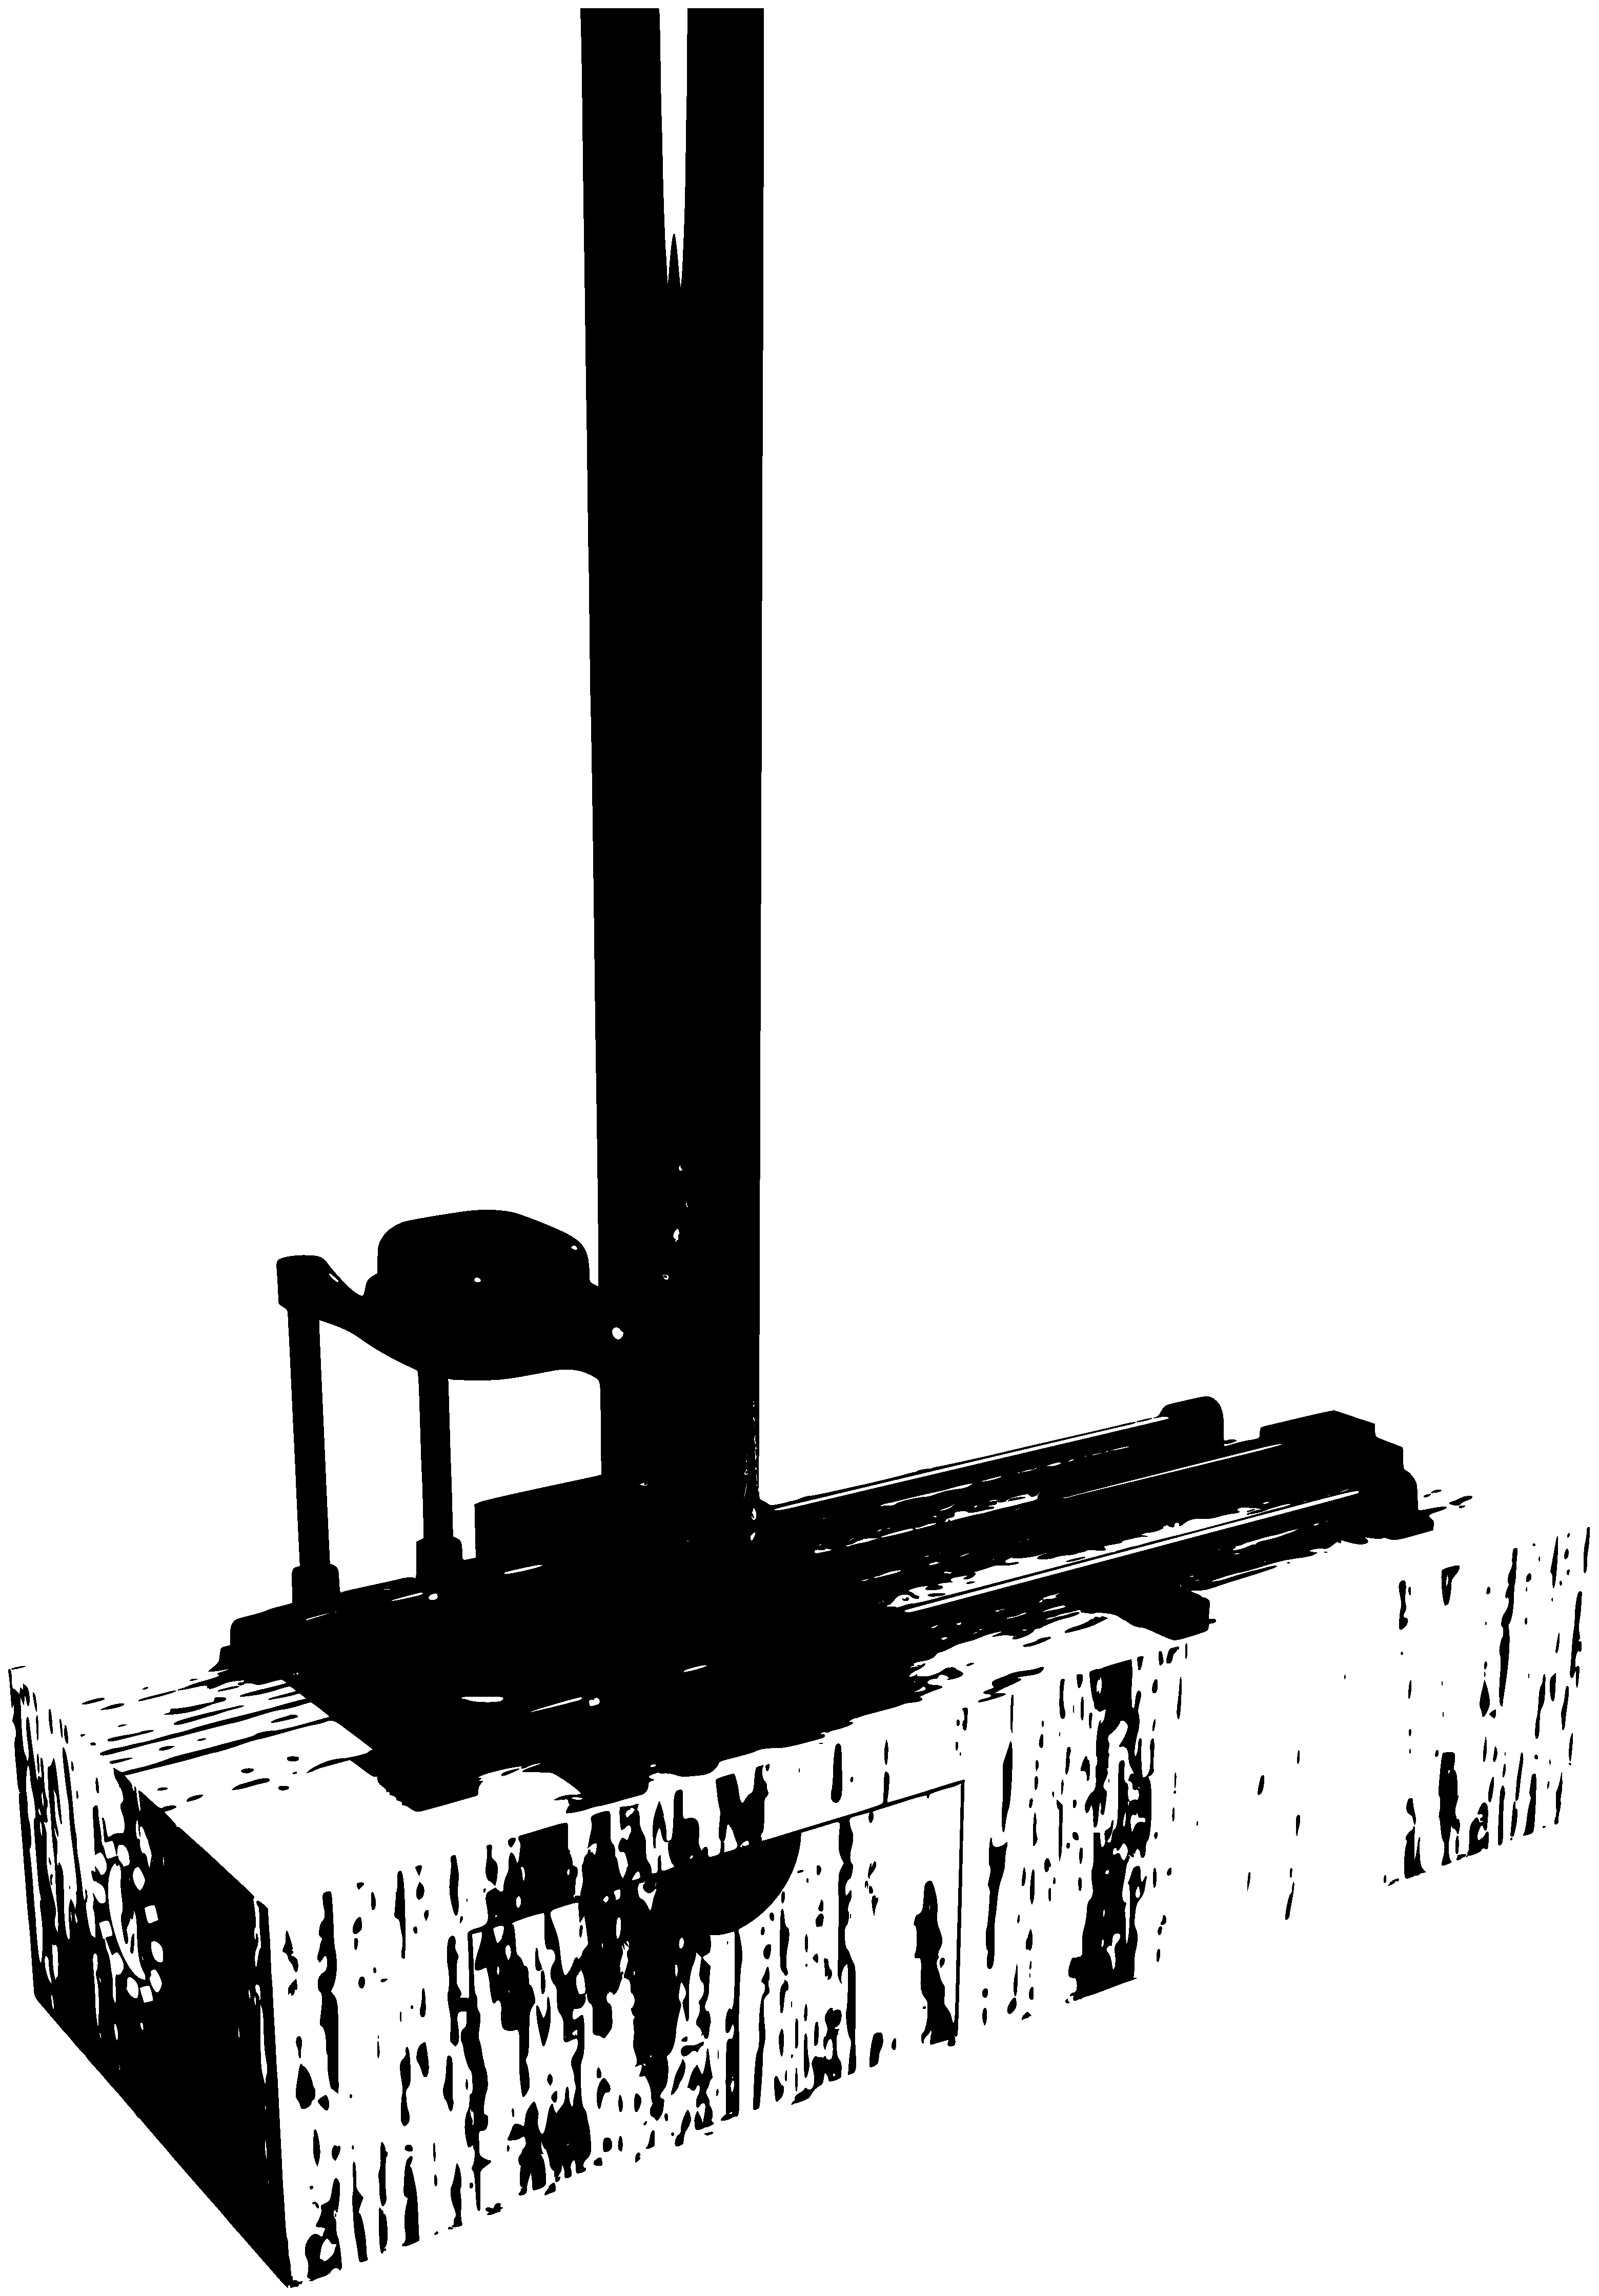
\includegraphics[width=\linewidth]{img/MachineCAO}
%	\captionof{figure}{Image 3D de la machine en fin de conception}
%\end{figure}


\subsection{Programmation des composants}
Avant de se lancer dans la programmation des composants, nous nous sommes assurés de leur bon fonctionnement en réalisant des tests unitaires.
On a ensuite programmé des fonctions de haut-niveau permettant de déplacer les Oréos, de faire pivoter le plateau, de contrôler l'allumage des LEDS, ... 
Nous avons intégré des sécurités dans ces fonctions pour éviter tout risque de casse : nous nous sommes servis de l'état des différents capteurs (switchs et détecteur de présence) comme condition de lancement des différentes actions. (Par exemple l'action "pousser un Oréo sur le plateau" nécessite que le capteur détecte le plateau en position horizontal).
A ce stade, on était donc en mesure faire défiler les Oréos en continu, mais pas encore de faire basculer le plateau selon leur classe car le programme qui s'occupe de la classification des Oréos ne tourne pas sur la carte Arduino.
On a donc dû mettre en place un système de messagerie pour que l'ordinateur et la carte Arduino puissent s'échanger des informations.

\section{Communication par le port Série (Entre le PC et l'Arduino)}
Pour faire communiquer le PC et la carte Arduino, on utilise un port série. On a défini un système de messagerie leur permettant de s'échanger des instructions.
Dans une première version de cette messagerie, on a créé une machine à état dans laquelle la réception ou l'envoi d'un certain message permettait de passer à l'état suivant.
Nous avons donc adapté nos codes C++ et Python pour que le poussage d'un Oréo par la machine déclenche la détection d'image de Python, que ce dernier renvoie sa décision (bon ou mauvais oréo) à la carte Arduino qui, elle, se charge ensuite de faire basculer le plateau du côté correspondant.
\\
Lors des premiers tests de cette messagerie, on s'est aperçu qu'aucun des messages envoyés, que ce soit par le PC ou la carte Arduino n'était reçu dans son entièreté. Après quelques recherches, nous avons compris que l'origine du problème était la vitesse de communication : initialement à 115200, nous avons réduit la vitesse à 57600 qui semblait enfin permettre une communication sans perte d'informations.
Nous avons alors pu lancer nos premières sessions de tri d'Oréo. Les résultats étaient plutôt concluants malgré quelques erreurs persistantes dans la détection.
Cependant nous avons remarqué que la machine restait parfois bloquée dans un état sans raison apparente, parfois très rapidement, d'autres fois après en avoir trié une vingtaine sans problèmes. Une inspection minutieuse du code nous a permis d'exclure la possibilité d'une erreur de programmation, en revanche nous avons retrouvé des messages présentant des pertes d'informations, ce qui expliquait la raison de ce blocage.
Nous avons alors entrepris de réaliser une messagerie plus robuste pour éviter cela. Nous travaillons en ce moment sur un système d'acquittement de messages et de vérification d'intégrité pour s'assurer de leur validité.





\section{Les prochaines étapes du projet}
Les prochaines étapes du projet sont les suivantes :
\begin{itemize}
	\item Améliorer le modèle de machine learning et résoudre le problème de sur-apprentissage.
	\item Continuer à travailler sur un modèle de reconnaissance des défauts par traitement d'image avec openCV. L'objecitf sera à terme de pouvoir executer deux modèles différents en parallèle pour avoir une décision plus fiable, ou au moins de pouvoir garder celui qui présente les meilleurs résultats.
	\item Rendre le protocole de communication plus robuste pour éviter les erreurs d'envois de messages.
	\item Réaliser l'interface graphique qui permettra d'interagir plus facilement avec la machine, avoir des informations sur l'état du programme et sur ce que voit la caméra.
\end{itemize}


%\section{Interface graphique}
%TODO



\end{document}
